\documentclass[a4paper,12pt]{article}

\usepackage{natbib}
\usepackage{times}
\usepackage{graphicx,epsfig}
\usepackage[leftcaption]{sidecap}
\usepackage{subfigure} % figures can have sub chunks
\usepackage{geometry} % this maxes page usage, making the below unnecessary
\usepackage{hyperref}
\usepackage{color}
\hypersetup{colorlinks=true, linkcolor=blue, filecolor=black,
  pagecolor=black, urlcolor=blue, citecolor=black}

\textwidth = 6.75in
\oddsidemargin = -0.25in
\textheight = 10in
\topmargin = -0.5in
\usepackage{fancyhdr}
\pagestyle{fancy}
\lhead{{\it Thomas AE. Smith }}
\chead{ }
\rhead{Coursework 2}
\lfoot{}
\cfoot{\thepage}
\rfoot{}

\newcommand{\goodgap}{%
 \hspace{\subfigtopskip}%
 \hspace{\subfigbottomskip}}

\title{Coursework 2: Understanding Social Behaviour in Games}
\author{Thomas AE. Smith}


\begin{document}
\maketitle

\section{Introduction}
This report describes the adaptation of a POSH agent for the Unreal Tournament 2004 game, in order to add additional capabilities that make it more effective in a capture-the-flag tournament environment. This involved developing code to specify a new behaviour, and modifying a provided basic plan in order to support the new behaviour and a range of new competences. The overall task was akin to a set of mid-development iterations of the BOD methodology.%, as in \citet{bryson2003behavior}.

% The Introduction should give a brief description of what you have done, and also give some idea about why you have done it (motivation). I expect you to cite a paper or two for the research context. For coursework 1, one of the papers you should probably cite is Brooks (1991), since you have been asked to take a fairly reactive approach to developing robot intelligence.

\section{Approach}
% The approach describes in detail exactly what you have done. This section is longer, and should ideally include some experiments you set up, for example to determine in what conditions you could get better results from the robot. The approach should be in sufficient detail that another person could replicate your experiments. You may cite other papers here too if you are taking an approach from another paper, or modifying it only slightly.
The first modification required by the specification was to add jumping capability to the agent. The provided agent was unable to jump over objects in its path, however the spawn point in the tournament map was gated by a low obstacle. Adding the new capability consisted of three tasks - providing code for the behaviour's actions and senses, adding these actions and senses to suitable locations within the agent's plan, and testing and debugging the implementation.

\subsection{Behaviours}
A new behaviour was developed, in order to provide the senses and actions required to support jumping over obstacles. Ideally from a design cohesiveness standpoint this functionality would have been added to the existing Movement.cs file, however the provided code could not be modified, and so the new code resides in a separate behaviour.

It transpired that the existing \texttt{IsStuck()} sense provided by Movement.cs was generally sufficient to indicate suitable trigger points for executing a jump action, and so the only code added was an action that sends a JUMP message.

\subsection{Plan}
In order to make use of the new action, a new drive element was added to the top of the drive collection --- i.e. with greater priority than any other element. Following this approach ensured that whenever the agent was moving for whatever reason, if it became stuck it would attempt to jump over whatever obstacle was blocking it. An alternative approach would have been to add the check and response to the \texttt{moveto-selected-nav} competence, however if alternate movement competences were to be added in the future, they would also need to duplicate the check and response.
\begin{description}
	\item[\texttt{jump-obstacle}:] If \texttt{IsStuck()} = 1.0, then follow the \texttt{jump-over} action pattern: send a JUMP message and reinitiate movement.
\end{description}

Aside from the ability to jump, a number of other competencies are needed for an effect tournament agent. The provided agent did not engage in combat and made no effort to retrieve its own flag if it was captured by the other team, and so elements were added to the plan in order to support these tasks. In decreasing order of priority:
\begin{description}
	\item[\texttt{return-our-flag}:] If our own flag is on the ground (it has been captured but the carrier was killed) return it to our own base in order to avoid having it recaptured. Select it as our navigation target, and move to it in order to return it.
	\item[\texttt{shoot-enemy-carrier}:] If our own flag has been captured, and we can see an enemy carrying it, shoot at that enemy. This element uses a provided sense and action from the Combat.cs class, and has a higher priority than capturing the enemy flag --- as without our own flag present at the base we cannot score.
	\item[\texttt{attack}:] If we can see an enemy, and we have both a gun and ammo, then select that enemy as a combat target and shoot at it for as long as we can see it. This has a lower priority than capturing the enemy flag, which allows for opportunistic attacks, but avoids pursuing enemies to the detriment of other goals.
\end{description}


\begin{figure}[h!]
	\centering
	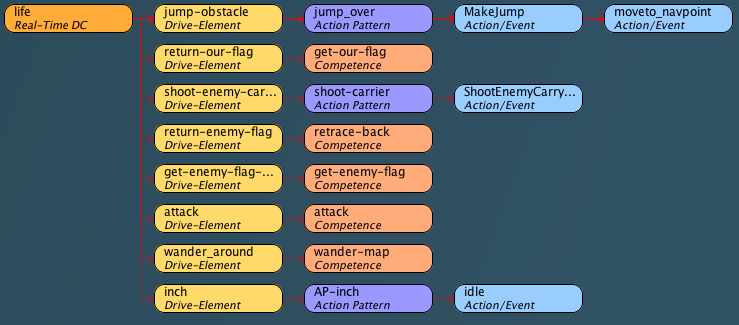
\includegraphics[width=\linewidth]{full}
	\caption{Overview of POSH plan}
	\label{fig:full}
\end{figure}

\section{Results}
Basic testing indicated that the modified agents performed better than the provided agents. On the provided testing map (\texttt{CTF-Bath-CW3-comp.ut2}), the low obstacle gating the spawn point completely blocked the original agents, which were unable to jump over it. On a version without the obstacles (\texttt{CTF-Bath-CW3-small.ut2}), the modified agents had an advantage due to the occasional opportunistic attacks against the non-violent provided agents. The provided agents also occasionally exhibited a bug where once killed they would thereafter not navigate properly --- this was fixed in the modified agents by removing references to \texttt{focusing\_task} from the \texttt{wander\_around} competence, and adding a \texttt{selected\_navpoint\_reachable} check.
% As with Coursework~1, please report experimental results, that is, propose and support hypotheses.  
% If you describe a reasonably-well working system in a comprehensible manner you will pass. If you can get the basic replication and describe it appropriately in the report, you will get around 55. Getting a mark over 70 requires demonstrating insight, creativity and/or understanding that goes beyond the basics laid out for you in this document.  You may want to read more papers on signal or language evolution, or the evolution of altruism (and obviously cite that reading).  However, only reference papers you really use in your research. 


% Describe what you attempted in order to get teamwork working, and the the impact of your strategy or strategies compared to single players and/or teams of identical, unmodified players.  It is quite possible that you may spend most of your space describing qualitative outcomes as a result of various approaches you have taken to the problem, but you can of course run tournaments between various strategies and report the outcomes.  Are they statistically significant? 

\section{Discussion}
% The discussion is the most discursive part of your paper, it may include speculation. You should discuss the extent to which your results addressed the questions described in your introduction, and what the results imply about your own work and work more broadly. You might suggest other experimental protocols that could have given different results and lessons learned. This can be a longer section as well.
The implemented additions to the behaviours and plan of the agent made it more suited to the capture-the-flag tournament environment --- however a number of other functionalities would also have been possible. The API supports the ability to be aware of and respond to incoming projectiles, or more advanced improvements such as improved pathfinding, varying agent roles or even inter-agent communication would potentially have improved the agents' overall performance. 

\section{Conclusion}
% The conclusion is just one paragraph. After possible digressions in the discussion, you should come back to state exactly what you tried to do (brief summary of the introduction), what the outcome was (brief summary of the results), and what you can certainly state as a result of this (the implications of the results in light of the introduction.)
The modified POSH agents were more effective in a capture-the-flag tournament environment than the provided POSH agents --- in some situations considerably so due to their ability to jump. The BOD methodology guided the development of iterative improvements to the agents' behaviours and plans, and made it easier to upgrade the provided code.

% \pagebreak

% \bibliographystyle{apalike}
% \bibliography{biblio}

\appendix
\section{Plan Modifications}\label{sec:app_plan}
\begin{figure}[h!]
	\centering
	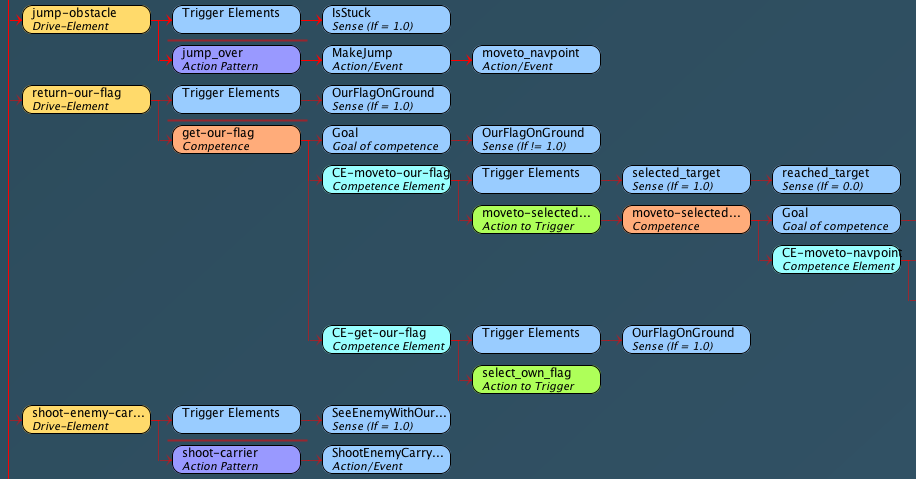
\includegraphics[width=\linewidth]{additions1}
	\caption{Jump and flag return behaviours}
	\label{fig:additions1}
\end{figure}

\begin{figure}[h!]
	\centering
	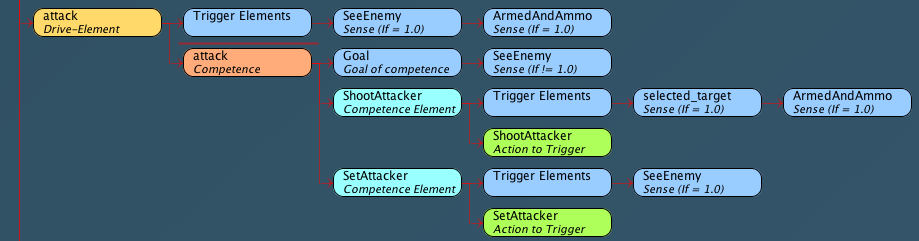
\includegraphics[width=\linewidth]{additions2}
	\caption{Attack-on-sight behaviour}
	\label{fig:additions2}
\end{figure}


\end{document}


\begin{figure}[h!]
	\centering
	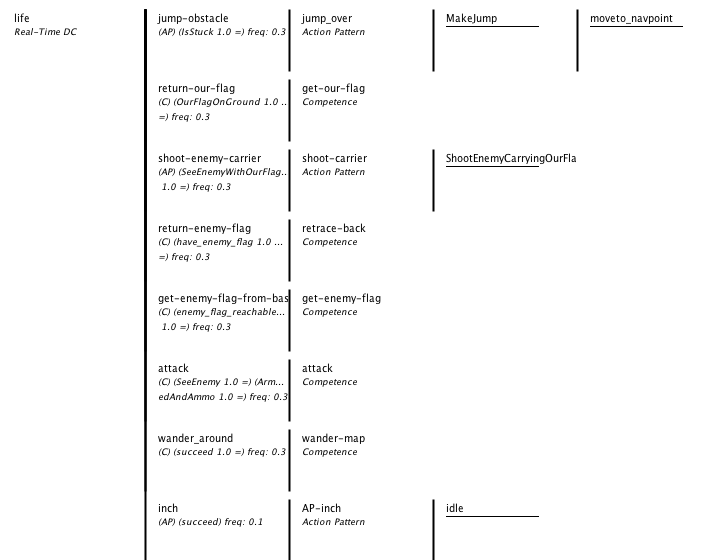
\includegraphics[width=\linewidth]{printview}
	\caption{Full plan}
	\label{fig:printview}
\end{figure}
